%------------
% directories
%------------

\def\FIGDIR{./figures}             % directory of pictures/diagrams
\def\TBLDIR{./tables}              % directory of tables
\def\CHAPDIR{./chapters}           % directory of chapters
\def\CODEDIR{./code}               % directory of code snippets
\def\STYDIR{./styles}              % directory of style files

%using memoir class for document preparations.
\documentclass[letterpaper,oneside,10pt,extrafontsizes]{memoir}

%Page setup
\settrimmedsize{11in}{210mm}{*}
\setlength{\trimtop}{0pt}
\setlength{\trimedge}{\stockwidth}
\addtolength{\trimedge}{-\paperwidth}
\settypeblocksize{8.0in}{33pc}{*}
\setulmargins{4cm}{*}{*}
\setlrmargins{1.0in}{*}{*}
\setmarginnotes{17pt}{51pt}{\onelineskip}
\setheadfoot{\onelineskip}{2\onelineskip}
\setheaderspaces{*}{2\onelineskip}{*}
\checkandfixthelayout

%packages
\usepackage{\STYDIR/mymadsen}
\usepackage{color,graphicx}
\usepackage{amssymb}
\usepackage{pifont}
\usepackage{longtable}
\usepackage[usenames,dvipsnames,svgnames,table]{xcolor}
\usepackage{hyperref}
\usepackage{colortbl}
\usepackage{array}

%styles
\headstyles{memman}
\chapterstyle{mymadsen}
\settocdepth{subsection}
\setsecnumdepth{subsection}
\makeindex[lines]
\tightlists
\midsloppy
\raggedbottom

%commands
\definecolor{ared}{rgb}{.647,.129,.149}
\renewcommand\colorchapnum{\color{ared}}
\renewcommand\colorchaptitle{\color{ared}}
\newcommand{\cmark}{\ding{51}}
\newcommand{\xmark}{\ding{55}}
\newcommand{\HorRule}{\color{black} \rule{\linewidth}{2pt}} % Defines the gold horizontal rule around the title

\listfiles

%%%%%%%%%%%%%%%%%%%%%%%%%%%%%%%%%%%%%%%%%%%%%%%%%%%%%%%%%%%%%%%%%%%%%%%%%%%%%%%%%%%%%%%%%%%%%%%%%%%%%%%%%%%%%%
%Document starts here
%%%%%%%%%%%%%%%%%%%%%%%%%%%%%%%%%%%%%%%%%%%%%%%%%%%%%%%%%%%%%%%%%%%%%%%%%%%%%%%%%%%%%%%%%%%%%%%%%%%%%%%%%%%%%%


\begin{document}
\frontmatter
\pagestyle{empty}
%----------------------------------------------------------------------------------------
%TITLE PAGE
%----------------------------------------------------------------------------------------

{\begingroup % Create the command for including the title page in the document
\hbox{ % Horizontal box
%\hspace*{0.2\textwidth} % Whitespace to the left of the title page
\rule{1pt}{\textheight} % Vertical line
\hspace*{0.05\textwidth} % Whitespace between the vertical line and title page text
\parbox[b]{2\textwidth}{ % Paragraph box which restricts text to less than the width of the page
{\noindent\Huge\bfseries {\color{brown}Scalable-Configurable AXI Switch (SCAS)} \\[4\baselineskip] \LARGE User Guide}\\[2\baselineskip] % Title
{\large \textit{V1.0 December 2013}}\\[4\baselineskip]
%{\Large \textsc{ARCHNTU}} % Author name

\vspace{0.5\textheight} % Whitespace between the title block and the publisher
{\noindent Nanyang Technological University, Singapore}\\[\baselineskip] 
}}
\endgroup}
\clearpage

{\begingroup
\parbox[b]{\textwidth}{
\hspace*{0.4\textwidth}
{\noindent\LARGE\bfseries {\color{red}NOTICE}} \\[2\baselineskip]
THIS DESIGN/HARDWARE/SOFTWARE IS PROVIDED BY THE COPYRIGHT HOLDERS AND CONTRIBUTORS "AS IS" AND
ANY EXPRESS OR IMPLIED WARRANTIES, INCLUDING, BUT NOT LIMITED TO, THE IMPLIED
WARRANTIES OF MERCHANTABILITY AND FITNESS FOR A PARTICULAR PURPOSE ARE
DISCLAIMED. IN NO EVENT SHALL THE COPYRIGHT OWNER OR CONTRIBUTORS BE LIABLE FOR
ANY DIRECT, INDIRECT, INCIDENTAL, SPECIAL, EXEMPLARY, OR CONSEQUENTIAL DAMAGES
(INCLUDING, BUT NOT LIMITED TO, PROCUREMENT OF SUBSTITUTE GOODS OR SERVICES;
LOSS OF USE, DATA, OR PROFITS; OR BUSINESS INTERRUPTION) HOWEVER CAUSED AND
ON ANY THEORY OF LIABILITY, WHETHER IN CONTRACT, STRICT LIABILITY, OR TORT
(INCLUDING NEGLIGENCE OR OTHERWISE) ARISING IN ANY WAY OUT OF THE USE OF THIS
APPLICATION, EVEN IF ADVISED OF THE POSSIBILITY OF SUCH DAMAGE.
PROVIDING THIS DESIGN, CODE, OR INFORMATION AS ONE POSSIBLE IMPLEMENTATION OF THIS FEATURE, 
APPLICATION OR STANDARD, WE ARE MAKING NO REPRESENTATION THAT THIS IMPLEMENTATION IS FREE FROM ANY
CLAIMS OF INFRINGEMENT, AND YOU ARE RESPONSIBLE FOR OBTAINING ANY
RIGHTS YOU MAY REQUIRE FOR YOUR IMPLEMENTATION.\\

REDISTRIBUTION AND USE IN SOURCE AND BINARY FORMS, WITH OR WITHOUT
MODIFICATION, ARE PERMITTED PROVIDED THAT THE FOLLOWING CONDITIONS ARE MET:\\ 
1. REDISTRIBUTIONS OF SOURCE CODE MUST RETAIN THE COPYRIGHT NOTICE, THIS
   LIST OF CONDITIONS AND THE DISCLAIMER.\\ 
2. REDISTRIBUTIONS IN BINARY FORM MUST REPRODUCE THE COPYRIGHT NOTICE,
   THIS LIST OF CONDITIONS AND THE DISCLAIMER IN THE DOCUMENTATION
   AND/OR OTHER MATERIALS PROVIDED WITH THE DISTRIBUTION.\\[2\baselineskip]   

Copyright \copyright~ 2013, ARCHNTU\\
* All rights reserved.
 
{\noindent The ARCH Research Group, Nanyang Technological University, Singapore\\
\url{http://arch.sce.ntu.edu.sg/}\\
contact: vipin2@ntu.edu.sg
}\\[\baselineskip] 
}
\endgroup}
\clearpage

\pagestyle{headings}
\tableofcontents*
\setlength{\unitlength}{1pt}
\clearpage
\listoffigures*
\clearpage
\listoftables*
\clearpage

\pagenumbering{arabic}

\mainmatter

\pagestyle{companion}

\chapter{Introduction}
\label{chap_intro}

Reconfigurable computing (RC) aims to fill the gap between hardware and software to achieve much higher performance than software, while maintaining a higher level of flexibility than hardware.
In order to achieve this performance benefit while supporting wide varieties of applications, reconfigurable systems are usually formed with the combination of reconfigurable logic and general purpose processors (GPPs).
Presently the most widely used reconfigurable logic in RC is the Field Programmable Gate Arrays (FPGAs) due to their high logic capacity, flexible routing architecture and wider tool support.
The reconfigurable logic implements custom hardware accelerators, which along with the software executed on the GPP provide much higher system performance compared to complete software implementations.

Although RC has been widely adopted in custom computing systems, it has not found acceptance into every day computing and scientific research.
Most of the custom RC applications are developed as standalone systems with very limited portability and reusability since there is no unified software and hardware communication interface for them.
Developers have to design communication and reconfiguration infrastructure even before testing the functionality of the target application.
This means there is lower productivity and longer design and implementation time.

Scalable-Configurable AXI Switch (SCAS) is an attempt to encourage the adoption of FPGA based accelerators on commercial computers.
This platform enables developers to quickly integrate hardware accelerators to a reusable communication as well as reconfigurable infrastructure capable of very high performance throughput. 
It supports PCIe, DRAM and Ethernet interfaces along with a configurable number of AXI-stream based communication channels to the user logic.
In addition to this, the user logic is also provided an address/data (PIO) interface for both PCIe and DRAM.
It allows run-time configuration of the communication pathways along with support for run-time reconfiguration of the user logic.
The hardware as well as software infrastructure is made completely open-source so that developers can adapt the platform to cater their specific requirements.
The present version is fully portable across Xilinx Virtex-6 FPGA based ML605 and Virtex-7 FPGA based VC707.
To enable this portability, some performance benefits of VC707 are sacrificed.
A high-performance platform will be released in the future exploiting the full capabilities of VC707.
\chapter{Installing SCAS}
\label{chap_installation}

The SCAS source files along with installation scripts can be downloaded from our public GIT repository \url{https://github.com/vipinkmenon/fpgadriver}.
The source file contains both the hardware as well as software components for SCAS.
The hardware components include all the source files for creating the FPGA configuration in verilog format, the Xilinx IP cores in synthesised (netlist) format, the constraints file for directing the FPGA place and route tools and some scripts for enabling command line execution of Xilinx development tools.
The software components mainly include the source file for the FPGA driver, the user library and a number of example applications.
The hardware development can be done on both Windows as well as Linux operating systems, but the SCAS FPGA driver is only supported on Ubuntu platform.

\begin{figure}[h]
\centering
\includegraphics[width=7cm]{figures/inst_hierarchy.pdf}
\caption{Directory Structure}
\label{inst_hierarchy}
\end{figure}

\noindent The hierarchy of SCAS components are shown in Fig.~\ref{inst_hierarchy} and described in Table~\ref{tab:hierarchy}.
The user library contains all the APIs required by the user application software to communicate with the hardware.
A single installation script is provided, which will install the Linux driver, user libraries and the ''hardware'' components.
To install the required file, switch the working directory into \emph{fpgadriver/install} and run the following commands.\\

\hspace*{4.45cm}{\texttt{chmod 777 install.sh}}\\
\hspace*{5cm}{\texttt{sudo ./install}}\\

Running script builds the driver and the user library. 
It then installs the driver and copies the user library (libfpga.so) to the shared user library location (/usr/lib/).
The installation also copies the hardware source files to a global location (/usr/include/fpga), so that the user application can access these components from any location similar to accessing the software shared library.
Once the installation is finished, the user software application can include the \emph{fpga.h} user library header file to use the driver APIs and can use \emph{-lfpga} as the library path during compiling.

\input \TBLDIR/hierarchy.tex

Use the example bitstream provided (v6\_top.bit or v7\_top.bit depending upon the target FPGA board) in the fpga/bitstream directory to program the FPGA for verification.
If you find difficulty in installing the Xilinx USB-JTAG cable for Ubuntu, follow the instructions at \url{http://www.george-smart.co.uk/wiki/Xilinx_JTAG_Linux#Newer_UDEV_.28Ubuntu_9.10.29}.
Reboot the host system since this is the first installation and the host needs to detect the board.
Now make sure that hardware is properly detected.
If you can visually inspect the board after rebooting, there should be 3 LEDs glowing and 1 LED constantly blinking.
\begin{itemize}
\item{LED0 : Blinking. Indicating Proper PCIe clock}
\item{LED1 : Internal PLL lock for DRAM}
\item{LED2 : PCIe link status}
\item{LED3 : DRAM link status}
\end{itemize}
It has been observed that ML605 board intermittently fails to detect DRAM.
In this case, power cycle the FPGA board, reprogram the FPGA and reboot.
To make sure that the host system has properly detected the FPGA board, execute the following command in the terminal\\
\hspace*{4.45cm}{\texttt{sudo lspci -vvv -d 10EE:*}}\\\\
lspci command lists the PCIe devices in the system and 0x10EE is the vendor ID for Xilinx.
This command will give detailed information about the configuration space of the FPGA PCIe endpoint.
The capability register values should indicate the device is Gen.2 capable and the link width is x4.
The control register indicates what is the configuration set by the host for the FPGA device.
For low-end host systems, the host may configure the device as only Gen.1 capable or in the worst-case as Gen.1 capable with only x1 link width.
This can severely affect the system performance.
If you have spare PCIe slots, try to plug-in the board to a different slot if this scenario occurs.

Make sure that the lspci command lists ''fpga'' as the driver for the endpoint device.
If the host fails to detect the driver, use the ''dmesg'' command to detect possible errors.\\\\
\hspace*{4.45cm}{\texttt{dmesg | grep fpga}}\\\\
If the hardware and driver installations are successful, go the application directory.
Run the \emph{fpga\_pio} example application by executing\\\\
\hspace*{4.45cm}{\texttt{./fpga\_pio}}\\\\
This should return the FPGA hardware version and the system health parameters.
The health parameter values are valid only on ML605 board since the VC707 board lacks the on-board sensors to measure these values.

Detailed description of integrating user applications and writing the application software are given in Chapters \ref{chap_integration} and \ref{chap_software}.
\chapter{Hardware}
\label{chap_hardware}

SCAS hardware provides programmable communication paths between different interfaces while maximising the throughput.
From an abstract point of view, SCAS can be seen as a form of crossbar switch (although not entirely true) interfaced with standard PCIe, DRAM, and Ethernet interfaces and a scalable AXI4-Stream based user logic interface.
The PCIe interface supports up to x4 PCIe Gen.2 standard, the DRAM interface supports up to 1GB DDR3-800 SODIMM modules and the Ethernet interface supports 1Gbit (Gigabit) raw Ethernet communication bandwidth.

\begin{figure}[h]
\centering
\includegraphics[width=8cm]{figures/switch.pdf}
\caption{Switch Architecture.}
\label{fig:switch_arch}
\end{figure}

\noindent The user interface supports 64-bit wide AXI4-Stream interfaces from both PCIe and DRAM (User PCIe Stream interface and User DRAM Stream interface).
The number of AXI4-Stream channels can be configured between 0 and 4 for both PCIe and DRAM.
The interface clock frequency to user logic for these stream interfaces are run-time reconfigurable and it defaults to 250MHz.
An abstract view of the switch architecture is given in Fig.~\ref{fig:switch_arch}.

The valid communication pathways for SCAS are shown in table~\ref{tab:cm_paths}.
The host system where the SCAS FPGA card is plugged in can directly communicate to the on-board DRAM and the user interface.
Presently communication through Ethernet is supported only from/to the DRAM.
Concurrent communication operations are possible and are managed within the FPGA logic and the driver software.
Generally user application does not have to bother about communication pathways interacting and causing data corruption or bottlenecks.
Some of the possible contention scenarios are described in Chapter~\ref{chap_integration}.
Detailed description of hardware modules are provided in the following sections.
For developing applications or using SCAS, users do not have to understand these low level details.
These are provided to encourage developers who would like to customise SCAS for their specific use cases.

\input \TBLDIR/communication_paths.tex

\section{PCIe manager}
The PCIe manager module manages all the data communication between the host system and the FPGA through PCIe interface.
The major sub-modules within this block are shown in Fig.~\ref{pcie_mnger}.
\begin{figure}[h]
\centering
\includegraphics[width=16cm]{figures/pcie_section.pdf}
\caption{PCIe Manager Architecture.}
\label{pcie_mnger}
\end{figure}

\subsection{PCIe Endpoint block}
This module uses the Xilinx PCIe Endpoint hard block configured in PCIe Gen.2 configuration with x4 link width.
This is the highest configuration supported in the Virtex-6 FPGAs although Virtex-7 devices supports PCIe Gen.2 in x8 configuration.
Theoretically PCIe x4 Gen.2 configuration can give a maximum throughput of 2GBytes/sec per direction in full-duplex mode.
The present configuration settings enable high-portability of user applications irrespective of the target FPGA.
The endpoint block implements the lower layers of PCIe protocol such as the data link layer and the physical layer.
The physical layer uses Xilinx's GTP tranceivers.
The maximum payload size for the PCIe core is set to 256bytes and the core uses 4 internal BRAM based buffers to store the PCIe packets.
The backend of the Endpoint is integrated with the fabric using AXI4-Stream interface to generate and consume PCIe packets from the upper layers.

\subsection{PCIe transaction layer}
The Endpoint block is directly interfaced with the receive and transmit engines, which act as the transaction layer for the PCIe protocol.
Transaction layer generates and consumes packets called transaction layer packets (TLPs), which are the unit of communication in PCIe.
The interface to the transaction layer is 64bits wide and runs at 250MHz clock frequency provided by the Endpoint.
The receive engine (Rx engine) decodes the received TLPs and route them to the appropriate sub modules.
The received TLPs may correspond to a memory read requests, memory write requests or a completion packets resulting from a memory read request issued by the FPGA.
If the memory write request is for an address location less than 0x400, it is routed to the global register set else it is directed to the user PCIe PIO interface.
Similarly for memory read requests, the request is forwarded to the global register or the user PCIe PIO interface depending upon the address and also triggers the transmit engine (Tx engine) to send the completion packet corresponding to this request with the data from the requested location.

From the completion packets, Rx engine extracts and packs the data and streams it out along with the \emph{tag number} in the received packet.
Tag number is a field in the PCIe packet inserted by a read operation initiator.
The device which responds to a read request should keep this same tag number in the completion packet, which enables the initiator to determine the specific request which generated this packet.
This is particularly useful when there are multiple outbound read requests.

The Tx engine generates TLPs corresponding to memory read, memory write and completion.
Memory read TLPs are generated during DMA operations to fetch data from host memory to the FPGA.
Memory write TLPs are generated while transmitting data from FPGA to the host memory and completion TLPs are generated in response to PIO read requests from the host.
The Tx engine also manages PCIe interrupts to the host (known as message signaled interrupt (MSI)) based on the request from the interrupt manager in the global register set.

\subsection{Global Register Set}
Table~\ref{tab:reg_set} lists the global register space of SCAS.
The PCIe endpoint device is configured to request for 4MBytes in the host system memory address space.
The first 0x3FC is reserved for the global register space and any access from the host above 0x3FC is routed to the user PCIe PIO interface.
If more memory space is required by the user application, the Xilinx PCIe endpoint IP has to be regenerated.
The details of regenerating the IP cores are described in Chapter~\ref{chap_customisation}.
Users are also free to add additional registers in the global set if required.

\input \TBLDIR/reg_set.tex

This module also implements the interrupt manager.
The interrupt manager makes sure that multiple back to back interrupts are not sent to the host in case of concurrent data transfer operations since this may sometimes crash the host or cause interrupt misses.
The manager queues the interrupt requests and clears the interrupts which are acknowledged by the host.
The host acknowledges interrupts by write clearing the status register (0x10) when it detects an interrupt.
\subsection{System Monitor}
System monitor is used to monitor the system health parameters such as temperature and power consumption.
It uses the Xilinx's System monitor hard macro along with on-board sensors.
These parameters can be accessed from the host system using an API (\emph{fpga\_read\_sys\_param()}).
The readings obtained from the System monitor are converted to actual values by the driver software using Xilinx specific transfer functions.
This monitoring functionality is available only on ML605 board since there are no on-board sensors on VC707 board.

\subsection{User Clock Generator}
This module generates the clock frequency used for all user stream interfaces.
There may be situations where the user logic cannot work at the system clock frequency.
This module takes the 250MHz clock from the PCIe core as the input and generates the output frequency depending upon an API request (\emph{user\_set\_clk()}).
Presently the supported output frequencies are 250,200,150 and 100MHz.
Internally this module uses the dynamic reconfiguration port (DRP) of an mixed-mode clock manager (MMCM) to derive the required clock frequency.
Using dedicated MMCM for user clock generation makes sure that other clock signals are not disrupted during clock reconfiguration.

\subsection{Multiboot Controller}
The multiboot controller (MBC) helps to reconfigure the FPGA by loading a new bitstream from the external storage memory (Platform Flash or BPI).
Internally the MBC instantiates Xilinx's ICAP primitive and uses the \emph{IPROG} command sequence to trigger a reconfiguration operation.
The application software uses the \emph{fpga\_reboot()} API to trigger a reconfiguration operation by specifying the starting address of bitstream in the memory.
The ML605 board is equipped with both Platform Flash as well as the BPI flash and VC707 board has only a BPI flash.
On VC707, while storing the bitstream in the BPI flash, it should be noted that the starting address-bitstream size combination should not cross 32MBytes since the BPI is partitioned into four region using the FPGA version selection pins.

\subsection{PCIe-DRAM DMA/PIO controller (PDMA)}
This module is responsible controlling data movement between the PCIe controller and the external DRAM memory.
This can access DRAM in both PIO (address/data) and DMA modes.
This module is configured by the registers in the global register space.
This module implements two virtual channels for host-DRAM write operations to achieve better performance.
In some applications PCIe write (host to FPGA) performance is lower due to some restrictions of the PCIe protocol.
As per PCIe standard, the maximum data that can be requested by an endpoint from the host in a single request is 4KB (or maximum read request size set by the host in the PCIe endpoint configuration space).
For large data transfers, this makes the endpoint to make several requests.
When an endpoint point makes multiple outstanding requests, the protocol provides the host the flexibility to return the completion packets in any order, irrespective of the requested order.
This is called out-of-order completion.
If the endpoint cannot manage this scenario, it is forced to make a new request only after receiving the data for the previous request.
This can severely affect system performance.
To overcome this issue, SCAS make use of the \emph{tag} number in PCIe packet.
Each time a memory request is made to the host, the request is tagged with a specific number.
As per the protocol, the completion packet returned for each request should maintain the tag number unaltered.
This enables reassembling data in correct order by PDMA.
Experiments showed that implementing only two such virtual channels will provide sufficiently high throughput performance.
Asymmetric FIFOs are used to convert 64bit wide PCIe interface data stream to 256bit wide DRAM interface data stream.

\subsection{PCIe Stream Generator (PSG)}
This module generates AXI-streams to the user PCIe-stream interface.
It is responsible for making data requests to the host system for transferring data from host to user stream interfaces and vice versa.
PSG instantiates asynchronous FIFOs between the user interface and PCIe data managers, which enables running the user PCIe stream interface at a different clock frequency than the PCIe core frequency.
The number of PSGs instantiated in SCAS depends upon the number of user PCIe stream interfaces specified by the user.
The FIFOs within PSGs are 8KB in size and a PSG never initiates a PCIe read or write operation unless there is sufficient buffer to store data.
This avoids creating deadlocks in the PCIe core.
For example if PSG requests for data without checking the space in the local FIFO and the user application stops receiving data from PSG, the PCIe core is stalled until the user application starts accepting data.

\subsection{PSG Stream Arbitrators (PSA)}
This module arbitrates among different PSGs.
It employs round-robin-arbitration among the streams to access the PCIe core controller.
It is highly scalable with current implementation supporting up to 256 PSGs.

\section{DRAM manager}
DRAM manger controls communication between the PCIe manager, user DRAM interface and the Ethernet manager with the external DRAM memory.
\subsection{DDR Controller}
This module instantiates the Xilinx's DDR3 soft memory controller.
It is generated using Xilinx's memory interface generator (MIG) available with the IP Core generator.
The controller is configured to control a 1GB DDRM SODIMM module running at 400MHz I/O clock frequency.
Its backend is a custom interface defined by Xilinx which is 256bits wide and runs at 200MHz.
\subsection{Four port memory controller (FPMC)}
This is the most important component of DRAM manager.
This module multiplexes DRAM access from different sources.
It has four identical ports which are interfaced to PCIe-DRAM DMA/PIO controller (PDMA), User DRAM PIO interface, User DRAM stream arbitrator (DSA) and the Ethernet manager.
Requests from these sources are served in round-robin-arbitration scheme.
Since the DDR controller has a single request port for access request, read-write request from each port is also served based on round robin.
For better system performance, FPMC allows back-to-back DRAM read requests and internally stores them in a tracking buffer.
When data is received from the DDR controller, it is routed to the appropriate port based on this tracking information.
\subsection{DRAM Stream Generator (DSG)}
DRAM stream generators control the DRAM-User logic AXI stream interfaces.
They are quite similar to PSGs except the fact that their user side interface is 64bits wide and DRAM interface side is 256bits wide.
Currently Xilinx does not support asymmetric (different read and write width) AXI Fifos.
Hence DSGs use two FIFOs with intermediate logic to convert interface widths.
The number of DSGs instantiated in the design depends upon the number of User DRAM stream interfaces specified by the user.
The FIFOs also enable the user DRAM stream interface to work at a different frequency than the DRAM core frequency.

\subsection{DSG stream arbitrator (DSA)}
DSG arbitrates requests from DSGs in a round-robin fashion.
DSG also implements a tracking buffer similar to the FPMC, which enables accepting back-to-back read requests from different DSGs.
\begin{figure}[t]
\centering

\includegraphics[width=16cm]{figures/ddr_arbitration.pdf}
\caption{DRAM Manager Architecture.}
\label{exe_model}
\end{figure}

\section{Ethernet manager}
The Ethernet manager control data movement between the DRAM manager and the Ethernet interface.
For Virtex-6, the Ethernet control used is a hard Tri-mode Ethernet MAC, where as Virtex-7 uses a soft Ethernet core.
The Virtex-7 Ethernet core requires special license from Xilinx for core as well as bitstream generation.
Ethernet manager has sub modules which perform Ethernet specified packing and unpacking of data and FIFOs and associated control logic to manage interface width mismatch.


\section{User Interface}
The user interface includes PCIe stream interfaces, DRAM stream interfaces, PCIe PIO interface, DRAM PIO interface and the interrupt interface.
The user interface signals are described in Table~\ref{tab:user_sigs}.

\input \TBLDIR/user_if_signals.tex

All the streaming interfaces (PCIe and DRAM) interface works at \emph{i\_user\_clk} frequency domain, whose default value is 250MHz.
The PCIe PIO interface as well as the interrupt interface works at the PCIe core frequency (250MHz).
The DRAM PIO interface works at DRAM core frequency, which is 200MHz.








\chapter{Integrating Accelerators}
\label{chap_integration}

The user logic (or the accelerator) should have an interface which has a subset of signals described in Table~\ref{tab:user_sigs}.
The user logic can have any number of sub modules, but the top most module name should be user\_logic\_top since it is the instantiation name used in SCAS.
If following command line implementation, three files are required for generating the final bitstream.\\
\begin{enumerate}
\item fpga\_spec.h~~~~~~~~~~~~~~~~~~~~~: The SCAS specification function
\item V6\_scas.tcl/V7\_scas.tcl ~~~~: Implementation TCL file
\item make\_fpga.sh~~~~~~~~~~~~~~~~~~~: Script to run the TCL file
\end{enumerate}
The specifications in fpga\_spec.h are given in Table~\ref{tab:spec}.
\input \TBLDIR/specs.tex
When enabling or disabling the Ethernet interface, a few things has to be noted.
For V6, the netlist for the Ethernet controller is installed in the global user library.
If the interface is disabled in the fpga\_spec.h file, the user has to set ENET\_ENABLE to 0 in the tcl file also.
This is to exclude the specific constraints used for Ethernet controller during implementation.
Otherwise this will cause errors in the ISE translate phase.
For V7, the Ethernet core has to be generated by the user with the name v7\_emac\_controller in SGMII standard.
This is since generating this core requires a special license from Xilinx and hence cannot be publically distributed.
The netlist for this core can be then stored in the global location or can be stored locally in the current working directory.

If the user logic is using sub modules, the names of these files have to be added in the tcl file using \emph{xfile add} attribute along with the presently listed files.
Additional constraints files can be also added in a similar manner.
Now execute the script make\_fpga with v6 or v7 as the argument depending upon the target board.
The script fetches all the required source, netlist and constraints files from the global location and also uses the local user logic files.
The final output will be top\_v6.bit or top\_v7.bit bitstream depending upon the target board.
Since the intermediate files share the same name, do not run the script concurrently for different boards from the same working directory.
\chapter{Software}
\label{chap_software}

The SCAS software comes with a software driver and a user library.
The driver implements all the low level device access files while the user library provides the APIs for high level data communication and system management.
When SCAS is installed, the user library is compiled as a shared library and is stored at the Linux shared user library directory.
This enables using these library functions from anywhere in the system by including the library header file (fpga.h) in the application software.
The APIs provided by the user library are listed in Table~\ref{tab:apis}.

\input \TBLDIR/apis.tex

From the API description, it could be seen that several APIs have of blocking and non-blocking attribute.
A blocking function is not returned until the operation is finished.
A non-blocking function returns soon after the operation is initialised but in this case the user has to synchronise the operation later by calling a synchronisation function (fpga\_wait\_interrupt()).
When the host is involved in data transfer, the blocking option is valid only when data is sent from host to the FPGA and not in the reverse direction.
For non-blocking data transfers from host, the maximum data chunk size for a single operation is 4MB.
Users must be careful while using blocking operations directly to the user logic as well as Ethernet interface.
If the host initiates a large data transfer directly to user PCIe stream interface in blocking fashion, and if the user interface is quite slow in accepting it, there can be significant performance loss.
Same applies to Ethernet data reception since it will be difficult to predict when the Ethernet data will be coming.

A potential dead lock when using block operation to user logic is when the user logic directly streams the processed data to the host.
If the user initiates a blocking write with a large data (more that what can be buffered within user logic and stream controllers), all the buffers gets filled up and the user application can not initiate a read operation since the write operation never exits without transferring the complete data.
For large data transfer operations, it is always encouraged to store the input data in DRAM and process it by reading from there and store the processed data back in the DRAM and later read back to the host.

\section{Software use cases}
This section describes the different use cases of communication between the host system and the fpga using different APIs. 

\subsection{FPGA PIO access}
The following example shows how to access the FPGA global registers using the PCIe PIO operations and get the system health parameters such as die temperature, FPGA core and I/O supply voltages, FPGA and board power consumption etc using the \emph{fpga\_read\_sys\_param()} API.
The \emph{fpga\_reg\_rd()} and \emph{fpga\_reg\_wr()} functions can be used to access the registers implemented in the user logic also.
It should be noted that all the registers in the user logic should have address equal to or above 0x400 since address space 0x00 to 0x3FC are used by the FPGA global register space.
The upper address limit for PIO access is 0x400000 limited by the present PCIe BAR0 configuration setting.
The complete address map for the fpga global registers is available in the driver header file (fpga.h).

\begin{verbatim}
#include <stdio.h>
#include "fpga.h"

int main() 
{
    sys_stat stat;                          //Structure returned by 
    int rtn;                                //fpga_read_sys_param function
    rtn = fpga_reg_rd(VER_REG);             //Read version register
    printf("Version : %0x\n",rtn);
    printf("Write scratch pad with 0x5\n"); //Write and read back scratchpad register
    rtn = fpga_reg_wr(SCR_REG,0x5);
    printf("Read scratch pad: ");
    rtn = fpga_reg_rd(SCR_REG);
    printf("%0x\n",rtn);   
    printf("Reading system parameters\n");
    stat = fpga_read_sys_param();           //returns the sys_stat structure,  
    printf("Temperature %f C\n",stat.temp); //which contains all the voltage,current,
    printf("VCCint %f V\n",stat.v_int);     //temperature and power information  
    printf("Vaux %f V\n",stat.v_aux);
    printf("V12s %f V\n",stat.v_board);
    printf("Iint %f A\n",stat.i_int);
    printf("Iboard %f A\n",stat.i_board);
    printf("FPGA Power %f Watt\n",stat.p_int);
    printf("Board Power %f Watt\n",stat.p_board);
    return 0;
}                 
\end{verbatim}


\subsection{DRAM PIO access}
The following example shows how to access the on-board DRAM memory location 0x1000 using PIO operations.
Both ML605 and VC707 are shipped with 1-GByte DDR3 memory.

\begin{verbatim}

int main() 
{   
    int rtn;
    rtn = fpga_ddr_pio_wr(0x1000,0xA5A5A5A5);  //DRAM PIO write to 0x1000 with 0xA5A5A5A5
    rtn = fpga_ddr_pio_rd(0x1000);             //DRAM PIO read from 0x1000
    return 0;
}
\end{verbatim}  


\subsection{Host to DRAM DMA}
The \emph{fpga\_transfer\_data()} API is used in the following example to transfer data from the host memory to the FPGA board DRAM.
In the API, the source is designated as the DMA source and DRAM as the destination.
The \emph{fpga\_malloc} API is used to get a free memory block in the DRAM.
The incremental data to be sent is pre-stored in an array which will be copied to the kernel memory space by the driver.
DMA between the host and the DRAM is always a blocking operation and hence the \emph{block} parameter has no effect in the API call.

\begin{verbatim}
#define DATA_POINTS (1024*1024)           //Size of current DMA write in bytes
unsigned int senddata[DATA_POINTS/4];     //Buffer to hold the send data

int main() 
{
    int rtn,i;
    unsigned int DRAM_ADDR;
    unsigned int arg = 0;
    unsigned int block = 0;
    
    DRAM_ADDR = fpga_malloc(DATA_POINTS); //Get the DRAM start address
    
    //Incremental Data for testing
    for(i = 0; i < DATA_POINTS/4; i++){
        senddata[i] = arg;
        arg++;
    }
    //Transfer the data
    rtn = fpga_transfer_data(HOST,DRAM,(unsigned char *)senddata,DATA_POINTS,DRAM_ADDR,block);
    rtn = fpga_free(DRAM_ADDR);
    return 0;
}
\end{verbatim}

\subsection{DRAM to host DMA}
This example shows how data can be transferred from DRAM back to the host.
It should be noted that the \emph{block} parameter has to effect in this case.
The function will return only after reading the complete data from DRAM.
\begin{verbatim}
#define DATA_POINTS (1024*1024)    //Size of current DMA read

unsigned int gDATA[DATA_POINTS];   //Buffer to hold the receive data

int main() 
{
    int rtn,i;
    long usecs;
    unsigned int DRAM_ADDR = 0;
    unsigned int block = 0;
    //Transfer the data
    rtn = fpga_transfer_data(DRAM,HOST,(unsigned char *)gData,DATA_POINTS,DRAM_ADDR,block);
    return 0;
}

\end{verbatim}

\subsection{Host to USER PCIe stream interface DMA}
This example shows how data can be directly send from the host to user PCIe stream interface with blocking option.
\begin{verbatim}

#define DATA_POINTS (64*1024*1024)  //Size of current DMA write
unsigned int senddata[DATA_POINTS/4];  //Buffer to hold the send data

int main() 
{
    int rtn,i;
    unsigned int arg = 0;
    unsigned int block = 1;

    //Incremental Data for testing
    for(i = 0; i < DATA_POINTS/4; i++){
        senddata[i] = arg;
        arg++;
    }
    //Transfer data in blocking mode
    rtn = fpga_transfer_data(HOST, USERPCIE1,(unsigned char *) senddata, DATA_POINTS ,0, block);
    return 0;
}
\end{verbatim}

This example shows how using the non-blocking capability enables sending data back-to-back from host to two different user PCIe stream interfaces.
Note how the synchronisation function is used at the end to sync. the operations.

\begin{verbatim}

#define DATA_POINTS (4*1024*1024)  //Size of current DMA write
unsigned int senddata[DATA_POINTS/4];  //Buffer to hold the send data

int main() 
{
    int rtn,i;
    unsigned int arg = 0;
    unsigned int block = 0;

    //Incremental Data for testing
    for(i = 0; i < DATA_POINTS/4; i++){
        senddata[i] = arg;
        arg++;
    }
    //Transfer data to User PCIe stream1 in non-blocking mode
    rtn = fpga_transfer_data(HOST, USERPCIE1,(unsigned char *) senddata, DATA_POINTS ,0, block);
    //Transfer data to User PCIe stream2 in non-blocking mode
    rtn = fpga_transfer_data(HOST, USERPCIE2,(unsigned char *) senddata, DATA_POINTS ,0, block);
    //Synchonise User PCIe stream1 transfer
    fpga_wait_interrupt(hostuser1);  
    //Synchonise User PCIe stream2 transfer
    fpga_wait_interrupt(hostuser2); 
    return 0;
}
\end{verbatim}

\subsection{USER PCIe stream interface to host DMA}

\begin{verbatim}
#define DATA_POINTS (1024*1024)  //Size of current DMA read
unsigned int gDATA[DATA_POINTS];  //Buffer to hold the send data

int main() 
{
    int rtn,i;
    unsigned int block = 0;
    rtn = fpga_transfer_data(USERPCIE1,HOST,(unsigned char *) gDATA,DATA_POINTS,0,block);
    return 0;
}   
\end{verbatim}

\subsection{USER DRAM stream interface to DRAM DMA}

\begin{verbatim}
#define DATA_SIZE 1024*1024  //Total number of bytes
int main() 
{
    int rtn,i;
    unsigned int block = 1;
    unsigned int DRAM_ADDR = 0x0;
    fpga_transfer_data(USERDRAM1,DRAM,DATA_SIZE,DRAM_ADDR,block);
    return 0;
} 
\end{verbatim} 


\begin{verbatim}
#define DATA_SIZE 1024*1024  //Total number of bytes
int main() 
{
    int rtn,i;
    unsigned int block = 0;
    unsigned int DRAM_ADDR = 0x0;
    fpga_transfer_data(USERDRAM1,DRAM,DATA_SIZE,DRAM_ADDR,block);
    fpga_transfer_data(USERDRAM2,DRAM,DATA_SIZE,DRAM_ADDR,block);
    fpga_transfer_data(USERDRAM3,DRAM,DATA_SIZE,DRAM_ADDR,block);
    fpga_transfer_data(USERDRAM4,DRAM,DATA_SIZE,DRAM_ADDR,block);
    //Synchonise transfers
    fpga_wait_interrupt(user1ddr);   
    fpga_wait_interrupt(user2ddr); 
    fpga_wait_interrupt(user3ddr); 
    fpga_wait_interrupt(user4ddr); 
    return 0;
} 
\end{verbatim}

\subsection{DRAM to USER DRAM stream interface DMA}

\begin{verbatim}
#define DATA_SIZE 1024*1024  //Total number of bytes
int main() 
{
    int rtn,i;
    unsigned int block = 1;
    unsigned int DRAM_ADDR = 0x0;
    fpga_transfer_data(DRAM,USERDRAM1,DATA_SIZE,DRAM_ADDR,block);
    return 0;
} 
\end{verbatim} 


\begin{verbatim}
#define DATA_SIZE 1024*1024  //Total number of bytes
int main() 
{
    int rtn,i;
    unsigned int block = 0;
    unsigned int DRAM_ADDR = 0x0;
    fpga_transfer_data(DRAM,USERDRAM1,DATA_SIZE,DRAM_ADDR,block);
    fpga_transfer_data(DRAM,USERDRAM2,DATA_SIZE,DRAM_ADDR,block);
    fpga_transfer_data(DRAM,USERDRAM3,DATA_SIZE,DRAM_ADDR,block);
    fpga_transfer_data(DRAM,USERDRAM4,DATA_SIZE,DRAM_ADDR,block);
    //Synchonise transfers
    fpga_wait_interrupt(ddruser1);   
    fpga_wait_interrupt(ddruser2); 
    fpga_wait_interrupt(ddruser3); 
    fpga_wait_interrupt(ddruser4); 
    return 0;
} 
\end{verbatim}         

\subsection{Host to USER DRAM stream interface DMA with buffering in DRAM}
This operation is supported only in blocking mode.
\begin{verbatim}
#define DATA_SIZE 1024*1024  //Total number of bytes
int main() 
{
    int rtn,i;
    unsigned int block = 0;
    unsigned int DRAM_ADDR = 0x0;
    fpga_transfer_data(HOST,USERDRAM1,DATA_SIZE,DRAM_ADDR,block);
    return 0;
} 
\end{verbatim}    

\chapter{Customisation}
\label{chap_customisation}
Users can customise SCAS for their specific application.
Additional registers can be implemented in the global register space by following the coding style and comments in the reg\_file.v verilog source file inside source/pcie\_if directory.
Another requirement will be to have more streaming interfaces to connect additional streaming peripherals.
This can be easily done by instantiating additional PSG and DSG modules (defined in pcie\_stream\_generator.v and dram\_stream\_generator.v).
These modules basically require information such as source and destination addresses, transfer length.
This can be done by implementing additional registers in global register space or in the user logic.
These modules use simple start/done control signals for operation.
They should be then integrated to the PSA and DSA for accessing the PCIe and DRAM cores.


\end{document}